%Author: Ashley Hill
%Attribution-NonCommercial 4.0 International (CC BY-NC 4.0) 

\documentclass{article}

\usepackage[margin=1in]{geometry} 
\usepackage{amsmath,amsthm,amssymb}
\usepackage[utf8]{inputenc} 
\usepackage{color}
\usepackage{tikz}
\usepackage{cancel}
\usepackage[linewidth=1pt]{mdframed}
\usepackage{pgfplots}

\usetikzlibrary{positioning}

\newcommand{\R}{\mathbb{R}}  
\newcommand{\Z}{\mathbb{Z}}
\newcommand{\N}{\mathbb{N}}
\newcommand{\Q}{\mathbb{Q}}
\newcommand{\C}{\mathbb{C}}

\newcommand{\argmin}{\operatornamewithlimits{argmin }}
\newcommand{\argmax}{\operatornamewithlimits{argmax }}

\newlength\tindent
\setlength{\tindent}{\parindent}
\setlength{\parindent}{0pt}
\renewcommand{\indent}{\hspace*{\tindent}}

\def\cunderline#1#2{\color{#1}\underline{{\color{black}#2}}\color{black}}
\def\cunderbrace#1#2{\color{#1}\underbrace{{\color{black}#2}}\color{black}}

\newcommand{\tikzmark}[1]{\tikz[baseline,remember picture] \coordinate (#1) {};}


\begin{document}


\title{Inférence Bayesienne \\ Cours 1}
\author{} 
\date{}

\maketitle

\section{Classification Baysienne}

$Y$: la classe à predire (catégorique)\\
$\vec{X}$: vecteur aléatoire, $\vec{X} = vec(X_1, ... X_d)$ \\

Choisir y qui maximise 

$$P(Y=y|\vec{X}=\vec{x}) = \left. \frac{\overbrace{P(\vec{X}=\vec{x}|Y=y)}^\text{vraisemblence} \overbrace{P(Y=y)}^\text{à priorie}}{\underbrace{P(\vec{X}=\vec{x})}_\text{évidence}} \color{red}\right] \color{red}\text{(niveau 1)} $$ \\

à estimé: $P(Y)$, $P(\vec{X}|Y) \rightarrow$ Pour chaque classe $y$ une distribution sur 
\begin{equation*}
 \vec{X} \xrightarrow[\text{(Hypothese naïve)}]{} P(\vec{X}=\vec{x}) = \prod^d_{i=d} \underbrace{P(X_i=x_i|Y=y)}_{\tikzmark{P}}
\end{equation*}
\begin{tikzpicture}[overlay,remember picture]
    \node (Ve) [below of = P, node distance = 2 em, anchor=west]{\footnotesize $\mathcal{N}(\mu_{iy}, \sigma_{iy}) (2\times K\times D)$};
    \draw[<-, in=180, out=-90] (P.south) to (Ve.west);

    \node (Vpe) [below right of = P, node distance = 1 em, anchor=west] {\footnotesize $\text{Bernoulli }\rightarrow \mathcal{O}_{iy} (K\times d)$};
    \draw[<-, in=180, out=-90] (P.south) to (Vpe.west);

\end{tikzpicture}
\vspace{1em}

\underline{Estimer les Parametres:}\\
\indent \underline{Cas Bernoulli:}
$$\mathcal{O}_{iy}=\frac{n(1,i,y)}{N(i,y)}$$\\
$$n(1,i,y) = \text{ nombre de fois où } X_i=1 \text{ dans la classe } y$$\\
Si $n(1,i,y) = 0 \Rightarrow \mathcal{O}_{iy}=0 \Rightarrow P(\vec{X}=\vec{x}|Y=y) = 0 \rightarrow \text{\underline{mal}}$ \\
Estimation MLE (Maximum Likleyhood Estimate) $\rightarrow$ frequentiste

\section{Inférence Bayesienne des paramètres (niveau 2)}

On cherche $P(X_i|Y) \rightarrow P(X_i|Y,\underset{\tikzmark{O}}{\underline{\mathcal{O}_{iy}}})$ 
\begin{tikzpicture}[overlay,remember picture]
    \node (Oe) [below of = O, node distance = 1 em, anchor=west]{\footnotesize \text{une variable aléatoire}};
    \draw[<-, in=180, out=-90] (O.south)++(0em, 0.5em) to (Oe.west);
\end{tikzpicture}
Apprendre le classifieur $\rightarrow$ estimer une distribution sur les paramètres\\ \\


\underline{Dans le 1):}\\
\xcancel{\indent MLE : $\mathcal{O}_{iy}$ maximise $P(\mathcal{D}|\mathcal{O}_{iy})$\\}

\vspace{1em}

\underline{Bayesien:} Estimer $P(\mathcal{O}_{iy}|\mathcal{D})$ \\
$$P(\mathcal{O}_{iy}|\mathcal{D}) = \frac{P(\mathcal{D}|\mathcal{O}_{iy})P(\mathcal{O}_{iy})}{P(\mathcal{D})}$$ \\

ex: Bernoulli, $P(\mathcal{D}|\mathcal{O}_{iy}) \rightarrow$ facile\\

\subsection{à priori sur les paramètres} 
bernouilli: $\mathcal{O}_{iy} \in [0,1]$, continue $\rightarrow P(\mathcal{O}_{iy})$ : une loi continue de support $[0,1]$ \\

le choix: loi Beta \\
\begin{mdframed}[linecolor=red]
$$P(\mathcal{O}_{iy}; \alpha_0, \alpha_1) = \underbrace{\frac{\Gamma(\alpha_0+\alpha_1)}{\Gamma(\alpha_0)\Gamma(\alpha_1)}}_{\text{Normalisation}} \underbrace{\mathcal{O}_{iy}^{\alpha_{1}-1}(1-\mathcal{O}_{iy})^{\alpha_{0}-1}}_{\text{}}$$\\
les parametres de la loi Beta $(\alpha_0, \alpha_1) > 0, \in \R$\\
\end{mdframed}

$\alpha_1=\alpha_0 > 1$\\

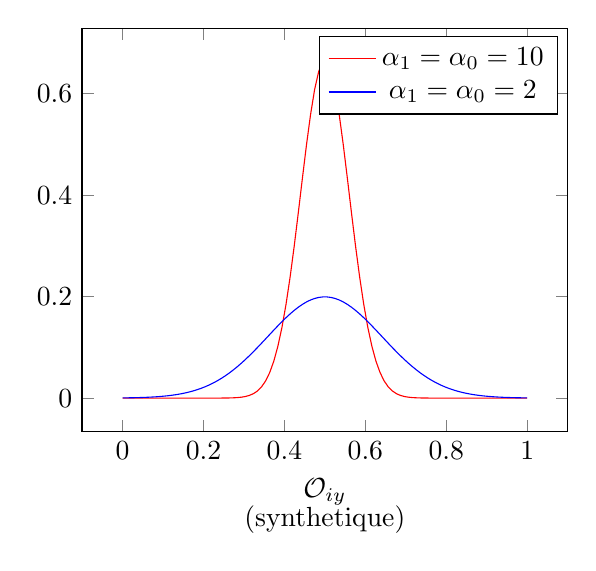
\begin{tikzpicture}
\begin{axis}[scale=0.9,title=(synthetique), xlabel=$\mathcal{O}_{iy}$, ylabel=, title style={at={(0.5,-0.2)},anchor=north},]
\addplot[domain=0:1, samples=100, color=red]{1/(0.06*sqrt(6.282))*exp(-(x-0.5)^2/(2*0.06^2))/10}; %1/(var*sqrt(6.282))*exp(-(x-avr)^2/(2*var^2))
\addlegendentry{$\alpha_1=\alpha_0=10$}
\addplot[domain=0:1, samples=100, color=blue]{1/(0.2*sqrt(6.282))*exp(-(x-0.5)^2/(0.2^2))/10}; 
\addlegendentry{$\alpha_1=\alpha_0=2$}
\end{axis}
\end{tikzpicture}
\\

\textbullet\underline{A priori non-informatif} \ ($\alpha_1 = \alpha_0=1$)\\

\begin{tikzpicture}
\begin{axis}[scale=0.9]
\addplot[domain=0:1, samples=100, color=blue]{1};
\draw[dotted] (axis cs:1,1) -- (axis cs:1,0);
\addplot[domain=1:2, samples=100, color=blue]{0}; 
\end{axis}
\end{tikzpicture}
\\

\textbullet\underline{A priori parcemonieux} \ (sparse)\\
$\alpha_1,\alpha_0<1$ \\

\begin{tikzpicture}
\begin{axis}[scale=0.9, scaled y ticks = false, ymax = 6]
\addplot[domain=0.01:0.99, samples=100, color=blue]{1/x+1/(1-x)-3.5};
\end{axis}
\end{tikzpicture}
\\

\subsection{à posteriori sur les paramètres} 
$$P(\mathcal{O}_{iy}|\mathcal{D}) \propto \underbrace{P(\mathcal{D}|\mathcal{O}_{iy})} \underbrace{P(\mathcal{O}_{iy};\alpha_1,\alpha_0)}_{\text{à priorie}} \\ \propto \underline{\mathcal{O}_{iy}^{N_1+\alpha_1-1} (1-\mathcal{O}_{iy})^{N_0+\alpha_0-1}}$$\\
$N_1(N_0)$ nombre de $x_i$ à $1(0)$ dans $\mathcal{D}$\\

La loi à posteriori est comme la loi à priori; une loi Beta.\\
\textcolor{red}{La loi Beta est l'a priori \underline{conjugé} de bernoulli. (Conjugated Prior)}\\

\subsection{Retour à la classification} 
a) \underline{Maximum à Posteriri des paramètres (MAP)} \\
\textcolor{red}{Dans le cas où $\alpha_0$ et $\alpha_1 > 1$}\\
$$\hat{\mathcal{O}_{iy}} = \argmax_{\mathcal{O}_{iy}} P(\mathcal{O}_{iy}|\mathcal{D}) \\ = \frac{N_1\tikzmark{Plus}+\alpha_1-1}{N_1+N_0+\alpha_1+\alpha_0-2}$$
\begin{tikzpicture}[overlay,remember picture]
    \node (Pluse) [below right=3em and 0.33em of Plus]{};
    \draw[red] (Plus.north)++(0.63em, 1em) to (Pluse.south);
    \node (leftPlus) [left=2em of Pluse, anchor=south]{\color{red}\text{$\mathcal{D}$(MLE)}};
    \node (rightPlus) [right=2em of Pluse, anchor=south]{\color{red}\text{à priori}};
\end{tikzpicture}
\vspace{2em}

\textbullet $\alpha_1$ et $\alpha_0$ agissent comme des \color{red}\underline{\color{black}"pseudo-comptes"}\color{black} $\rightarrow$ lissage (smoothing) de distribution \\
\textbullet $\mathcal{O}_{iy} \neq 0$ \\
\textbullet Si $N_1$,$N_0$ $>> \alpha_1$,$\alpha_0$ l'a priori negligable $\rightarrow$ Régularisation, écrit sur-apprentissage\\

b) \underline{Loi predictive (inférence Bayesienne 3)} \\
$$P(X_i=x_i|Y=y;\tikzmark{O2}\mathcal{O}_{iy})$$ \\
\begin{tikzpicture}[overlay,remember picture]
    \node (O2e) [below right of = O2, node distance = 2 em, anchor=west]{\footnotesize \text{estimer à partire de $\mathcal{D}$ (MAP)}};
    \draw[<-, in=180, out=-90] (O2.south)++(1em, -0.5em) to (O2e.west);
\end{tikzpicture}

La vraie prédiction: $$P(X_i=x_i|\mathcal{D}) = \int_{0}^{1} P(X_i=x_i,\mathcal{O}_{iy}|\mathcal{D}) d\mathcal{O}_{iy}$$ 
$\rightarrow$ en marginalisant les paramètres. \\

$$\cunderbrace{red}{P(X_i,\mathcal{O}_{iy}|\mathcal{D})} = \color{red}\underbrace{\color{black}P(X_i|\mathcal{O}_{iy},\mathcal{D})}_\text{\color{black}vraisemblence}\ \color{red}\underbrace{\color{black}P(\mathcal{O}_{iy}|\mathcal{D})}_\text{\color{black}2.2)}$$ \\
$$P(X_i=1|\mathcal{D})=\frac{N_1+\alpha_1}{N_1+N_0+\alpha_1+\alpha_0} ~~~ ,\forall\alpha_1\text{ et }\alpha_0 > 0$$\\

\end{document}
